\chapter{Conceito do Sistema}
\label{chap:concep}

\begin{flushright}

   \begin{list}{}{
      \setlength{\leftmargin}{4.5cm}
      \setlength{\rightmargin}{0cm}
      \setlength{\labelwidth}{0pt}
      \setlength{\labelsep}{\leftmargin}}
      \item Quanto maior for a rapidez de transformação de uma
      sociedade, mais temporárias são as necessidades
      individuais. Essas flutuaçõess tornam ainda mais acelerado
      o senso de turbilh da sociedade.

      \begin{list}{}{
      \setlength{\leftmargin}{0cm}
      \setlength{\rightmargin}{0cm}
      \setlength{\labelwidth}{0pt}
      \setlength{\labelsep}{\leftmargin}}
      \item (Alvin Toffler)
      \end{list}
   \end{list}
\end{flushright}

\begin{flushright}
  Quanto maior for a rapidez de transformação de uma \\
  sociedade, mais temporárias são as necessidades \\
  individuais. Essas flutuações tornam ainda mais \\
  acelerado o senso de turbilhão da sociedade. \\
  \ \\
  (Alvin Toffler)
\end{flushright}

%--------- NEW SECTION ----------------------
\section{Estudo do estado da arte}
\label{sec:sota}
flkjasdlkfjasdlkfjs

%--------- NEW SECTION ----------------------
\section{Descrição do sistema}
\label{sec:desc}
lasdjflsadjf

\subsection{Especificação técnica}
\label{ssec:espt}
lakjfldksjfdslakjf

\subsection{Arquitetura geral do sistema}
\label{ssec:arqg}
lkasjdflksdajflk;

\subsubsection{Arquitetura do sistema de movimentação}
De forma a garantir uma movimentação efetiva do robô é necessária a integração de diversos ferramentas físicas e de software, como a estrutura de movimentação adequada, sistema ordenamento de missão, controle de potência,demandando assim um \textit{framework} e um sistema operacional.

A inspeção de linha foi denominada missão, para cade vez que o robô começar a realizar a inspeção, será considerado o início de uma nova missão. 

Para garantir a execução correta da missão e ultrapassagem dos obstáculos de forma efetiva, se dividiu o sistema em 4 principais subsistemas, sendo elas : \textit{Motion Planning} , \textit{Actuation},\textit{System Integrity Check} e \textit{Power Management}. A arquitetura geral do sistema de movimentação está mostrada na figura \ref{fig:arq_geral}, ilustrando os subsistemas e suas funcionalidades. 
\begin{figure}[h]
	\centering
	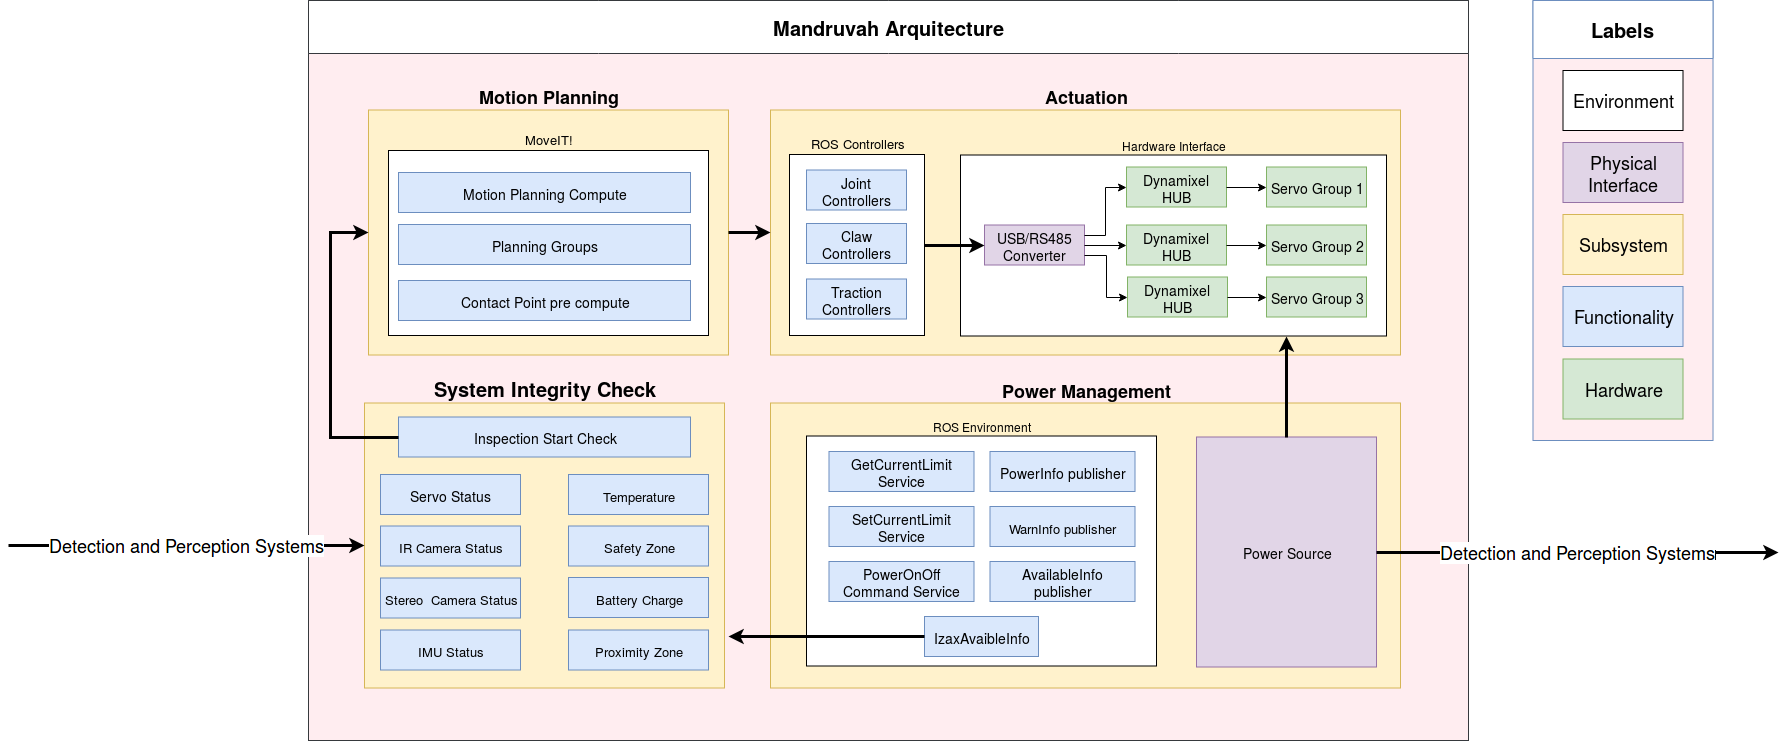
\includegraphics[width=1\textwidth]{Arquitetura.png}
	\caption{Arquitetura Geral do sistema de movimentação}
	\label{fig:arq_geral}
	\source{Própria}
\end{figure} 
A estrutura física do robô foi projetada para que sejam realizados movimentos de translação e transposição de obstáculos presentes na linha de transmissão,consistindo de unidades de tração para a translação na linha e juntas nos braços e garras para a realização da ultrapassagem de obstáculos. O controle da estrutura física do robô está relacionado com a \textit{Actuation}.
A transposição dos obstáculos é um grande desafio para essa aplicação, visto que será necessário a aplicação da cinemática inversa no robô. A cinemática inversa consiste num conjunto de equações que definem o movimento do robô para a movimentação de um ponto à outro, tal modelo é extraído à partir da estrutura do robô. A funcionalidade responsável por calcular esse modelo e encontrar como será feita a movimentação foi denominada \textit{Motion Planning}.
Para garantir a execução correta da missão e preservar a integridade do robô foi estipulada uma funcionalidade que checa os dispositivos antes de cada missão, denominada \textit{System Integrity Check}. E com a finalidade de realizar o controle da potência no robô foi será utilizado o projeto de uma placa específica para esse papel, assim todos os aspectos relacionados à alimentação do robô, assim como consumo e monitoramento estão atrelados ao \textit{Power Management}.

O \textit{framework} ROS possibilita a integração de todas essas funcionalidades, sua estrutura baseada em nós facilita a identificação dos problemas e possibilita a modularização do código. Fornecendo também diversas ferramentas como o \textit{MoveIt!}, que será utilizada para o \textit{Motion Planning}, assim como drivers de compatibilização para os servo motores adotados no projeto.

\subsection{Arquitetura de software}
\label{ssec:arqs}

%--------- NEW SECTION ----------------------
\section{Desdobramento da função qualidade}
\label{sec:qfd}
asdfsdafsf

\subsection{Requisitos técnicos}
\label{ssec:reqt}
asdfsadfdsf

